\documentclass[review,numbers,sort&compress]{elsarticle}  %10pt,

\usepackage{lineno,hyperref}
\linenumbers
\modulolinenumbers[5]
\usepackage{times}
\usepackage{amsmath}
\usepackage{amssymb}
\usepackage{epsfig}
\usepackage{epstopdf}
\usepackage{graphicx}
\usepackage{makecell}

\usepackage{booktabs}
\usepackage{multirow}
\usepackage{dcolumn}
\usepackage{threeparttable}
\usepackage{setspace}
\usepackage{algpseudocode}
\usepackage{algorithm}
\usepackage{color}
\usepackage{array}
\usepackage[table,xcdraw]{xcolor}

\usepackage{graphicx}
\usepackage{subfigure}



\journal{Journal of \LaTeX\ Templates}

%\bibliographystyle{elsarticle-num-names}
%\bibliographystyle{plain}
%\bibliographystyle{elsarticle-harv}

%% Numbered
%\bibliographystyle{model1-num-names}

%% Numbered without titles
%\bibliographystyle{model1a-num-names}

%% Vancouver name/year
%\usepackage{numcompress}\bibliographystyle{model4-names}%\biboptions{authoryear}

%% APA style
%\bibliographystyle{model5-names}%\biboptions{authoryear}

%% AMA style
%\usepackage{numcompress}\bibliographystyle{model6-num-names}


\begin{document}

\begin{frontmatter}

\title{Extreme Learning Machine based Single Image Super Resolution}

%\renewcommand{\thefootnote}{\fnsymbol{footnote}}



\begin{abstract}
Although Convolution Neural Network(CNN) based methods have recently become popular for image super-resolution, most of them are time-consuming and computationally complex. It is difficult to apply those methods to real-time applications or devices with low compute capability. In this paper, we propose a novel method for fast single image super-resolution. We use a decision tree to divide image patches to different subspaces fast. Patches divided into same subspace suppose to be similar and it is accurate and efficient to learning a mapping function from Low-Resolution(LR) space to corresponding High-resolution(HR) space. Extreme Learning Machine(ELM) is a fast learning algorithm because its special traits. We use ELMs to learn mapping functions for every subspace. All subspaces mapping models and the decision tree form a piece-wise non-linear function. Extensive experiments on benchmark datasets show that the utility of the proposed method for image super-resolution in speed and accuracy.
\end{abstract}

\begin{keyword}
Single image super-resolution\sep Extreme Learning Machine\sep Decision tree
\end{keyword}
\end{frontmatter}



%----------------------------------Introduction-----------------------------------
\section{Introduction}

Image super-resolution is to reconstruct a high resolution from one or more given low resolution image. Lots of high frequency information such as tiny textures is lost in low-resolution image, which makes SR problem highly ill-posed. Image super-resolution plays an important role in many fields, such as video surveillance, remote sensing and image sensing. The Eq.~\ref{eq:form_low_H} shows the relationship between low-resolution images and its high-resolution image.
\begin{equation}\label{eq:form_low_H}
   X = HY+n
\end{equation}
where $H$ is the down-sample kernel, and n is the noise. The low-resolution image $X$ is derived from its origin image, which is down-sampled and noised. In general, single image super-resolution methods can be divide into three categories: interpolation-based method, learning-based SR methods and reconstruction-based SR methods.

The simplest super-resolution (SR) method is the interpolation-based method. This kind of SR method uses a linear kernel to filter the input LR image to obtain the HR image. The interpolation kernel is single and low-pass, thus it can not estimate the potential image structure. In addition, the information provided by the input LR image is limited, which causes the smoothness in the output HR image. Thus, the interpolation-based methods can not satisfy the reality needs.

The learning-based SR methods learn the mapping relationship between the LR space and HR space to address the SR problem. Most existing learning-based methods can classify into two classes: the coding-based methods and the regression-based methods. The coding-based methods assume that there exists isometric manifolds in the coupled LR-HR space. This assumption allows encoding coefficients in LR space to be directly passed to the corresponding HR space. Then, they are used for SR reconstruction. Lu et al. proposed an SR method based on locally linear embedding \cite{chan2007superresolution}. The SR method proposed by Gao et al. combines sparse representation and neighborhood embedding \cite{lu2013image}. The sparse-coding-based SR methods construct the corresponding dictionary from the LR space and the HR space, respectively. The LR dictionary is used to compute the encoding coefficients for the input LR feature. Then, the coefficients can be used directly in the HR dictionary. The target HR output is obtained by computing the weighted sum of the HR dictionary atoms. According to the way the dictionaries are constructed, the sparse-coding-based SR methods can also be classified into two categories: the orthogonal dictionary based methods \cite{mallat2010super}\cite{dong2013sparse} and the over-complete dictionary based methods \cite{yang2010image} \cite{yang2012coupled}\cite{lu2014alternatively}\cite{wang2012semi}. The regression-based SR methods directly learn the mapping from the LR space to HR space. The SR method proposed by Freeman et al. uses the Markov random field (MRF) \cite{freeman2000learning}. Kim et al addressed the SR problem by sparse representation and kernel regression \cite{kim2010single}. Moreover, there are SR methods based on linear regression \cite{yang2013fast}\cite{zhang2015learning}, SVM regression \cite{ni2007image}, and Gaussian process regression \cite{wang2017single}\cite{he2011single}\cite{li2015learning}\cite{wang2016image}

The reconstruction-based SR methods \cite{IRANI1991231}\cite{1033210} \cite{lin2004fundamental}use multiple LR images to reconstruct an HR image. These LR images all come from the same scene, and there must be sub-pixel shifts between them. In real, users may not necessarily obtain multiple LR images that meet this requirement. Thus, its application is limited.

Some researchers train a deep convolution neural network to learn the mapping model from the LR space and HR space \cite{kim2016accurate} \cite{kim2016deeply} \cite{lai2017deep} \cite{shi2016real}. This type of SR methods greatly improve the image SR. However, the training process is complicated, and it involves a longer training time. Based on the obstacles of training neural network and the advantages of extreme learning machine (ELM), we propose an ELM-based single-image SR method. The proposed method employs the piecewise non-linear regression scheme. First, it conducts Hadamard transform on LR training data (LR training image patches) to obtain Hadamard patterns. Then, the training data (LR-HR training image patch pairs) are classified based on the generated Hadamard patterns. Last, each subspace is used to train a mapping model, which is a non-linear mapping model from the LR space to HR space, ELM. All of the mapping models form a piecewise non-linear SR function. Our method also employs the ternary decision tree. Experimental results show that the proposed method yields competitive objective evaluation results and better subjective reconstruction results at the fastest running speed.

The remainder of this paper is organized as follows:Section \uppercase\expandafter{\romannumeral2} introduce the related work of algorithms about image super-resolution. Section \uppercase\expandafter{\romannumeral3} describe the fundamental concepts and theories of ELM. Section \uppercase\expandafter{\romannumeral2} presents the proposed method. Section \uppercase\expandafter{\romannumeral5} gives the experiment results on different datesets and the visual comparisons with other methods are also included. Finally, Section \uppercase\expandafter{\romannumeral2} draws conclusions.


%------------------------------------Related Work---------------------------------
\section{Related Work}
ELM is used for training a single-hidden-layer feed-forward network, and some researchers tried to use it for HR image reconstruction \cite{an2012image} \cite{sidike2017fast} \cite{cosmo2017single}. The ELM-based single-image SR method was first introduced in \cite{an2012image}. This method firstly interpolates the input LR image to the desired size.  Then, it extracts the first-order and second-order gradients from the interpolated image as high-frequency features. After that, a traditional ELM is used to perform the regression operation. The mapping relationship between the LR input and the high-frequency feature is learned. For HR reconstruction, this method only considers gradient information in horizontal and vertical directions. Compared with the method in\cite{an2012image}, the algorithm in \cite{sidike2017fast} extracts gradient information in more directions. This algorithm uses the Robinson compass operator as the derivative filter, and it rotates the single kernel in eight directions. The eight newly generated kernels are used to extract the input LR image’s gradient information in eight directions. The extracted information is used to predict the missing high-frequency details. In this method, more directional information improves the reconstructed accuracy.

The above two methods address the single-image SR problem by a global mapping model. The literature \cite{cosmo2017single} starts with the initial idea of the literature \cite{an2012image}, and it trains multiple mapping models to reconstruct the HR image. This algorithm computes directional features based on all the pixel positions in an image patch. Then, the dimensionality of directional features is decreased by PCA. In the training phase, this method first clusters the training data by K-means. For each cluster, a mapping model is calculated by ELM, and it is a non-linear mapping model from the LR space to HR space. In the testing phase, the cluster centroid with the minimum distance to the LR image patch is first found. Then the corresponding mapping model is used to generate the HR image patch. All of the generated HR image patches form the target HR output.

The three ELM-based SR methods \cite{an2012image} \cite{sidike2017fast} \cite{cosmo2017single} learn the non-linear mapping models from the LR space to HR space, by which the reconstructed HR is generated. Recent years, some regression-based single-image SR methods have also achieved good results.

Timofteet et al. proposed  ANR method \cite{timofte2013anchored} and A+ method \cite{timofte2014a+}, and the A+ method is the improved version of the ANR method. Both of them adopt the piecewise linearization scheme. Timofteet et al. assumed that the mapping between the LR space and HR space is locally linear. Thus, many linear regressors are learned and anchored to the feature space. The ANR and A+ methods use the sparse dictionaries in a different way, whereby the process of computing encoding coefficients is token place by choosing the anchored point. This change increases the running speed and improves the reconstruction accuracy. Tang et al. employed the sparse coding and the structured output regression machine (SORM) to learn the non-linear mapping relationship between the LR feature space to corresponding HR feature space, whereby a global non-linear optimization model is adopted to improve the accuracy.

The SR methods in \cite{huang2017learning} \cite{huang2015practical} \cite{huang2015fast} \cite{schulter2015fast} \cite{xiong2018gradient}are decision-tree-based, whereby the random forest is comprised of multiple decision trees. All the methods in\cite{huang2017learning}\cite{huang2015practical}\cite{huang2015fast}\cite{schulter2015fast} construct an SR decision tree. Each leaf node of the SR decision tree is corresponding to a linear mapping model from the LR space to HR space. The method in \cite{huang2017learning} uses all the training data to initialize the root node of the decision tree, then it progressively constructs an SR decision tree with a hierarchical structure. The methods in \cite{huang2015practical}\cite{huang2015fast}\cite{schulter2015fast} first divide the training data into many subsets, each of which is used to construct an SR decision tree. All the SR decision trees form the SR random forest. Both the generated SR decision tree and the SR random forest represents a piecewise linear SR system respectively. Xiong et al. learned the mapping model by a multi-output gradient boosting framework, whereby the decision tree is used as a basic learner. In this method, the learning process of the SR decision tree is guided by gradient boosting.

Methods in \cite{dong2016image}\cite{lai2017deep}\cite{tai2017image} are all based on convolutional neural network. \cite{dong2016image} has a simple network structure of three layers, whose training time approximates to three days. The method in \cite{tai2017image} employs the residual learning to reduce the difficulty of training a deep network. When the depth of the network increases, this method uses the recursive learning to control the number of the parameters of network. The feature extraction branch consists of many convolutional layers and a transposed convolutional layers, which upsamples the extracted features by a upscaling factor of two. In the reconstructing phase, the input LR image is first upsampled, then the upscaled image is added to the predicted residual image to generate the HR image. The LR image is progressively upsampled, whereby the traditional bicubic interpolation algorithm is replaced by a transposed convolutional layer.

The convolutional-neural-network-based SR methods have greatly improved the reconstruction accuracy. They can estimate the complicated non-linear mapping directly from the input samples. However, the training time is too long. In addition, all the parameters are tuned during the training process. The popular learning algorithm for convolutional neural network is back propagation. It can effectively calculate the gradient by passing the output forward to the input. However, there are some problems. The smaller learning rate will leads to slower convergence speed, and the bigger learning rate will result in instability and divergence. Moreover, the back propagation may convergence to a local minimum. Overtraining can also leads to poor generalization performance.

Compared with back propagation, ELM’s training speed is much faster. The proposed single-image SR method learns the non-linear mapping relationship between the LR space and HR space using ELM. Experimental results show that the reconstructed images by our SR method are much closer to the original HR images, and the proposed method has a much faster running speed.


%------------------------------------ELM---------------------------------
\section{Extreme Learning Machine (ELM)}
Extreme learning machine (ELM) is a fast learning algorithm for training a single-hidden-layer feedforward neural networks (SLFNs) \cite{huang2004extreme}\cite{huang2006extreme}\cite{huang2012extreme}. One of its advantages is that we don not need to tune the parameters of hidden layer. Moreover, the weights of the output layer can be calculated through a closed form solution.
For a generalized single-hidden-layer feed-forward neural network, the output function of one node is formulated as
\begin{equation}\label{eq:SLFNS}
  f(x)=\sum_{i=1}^{L}\beta_i h_i(x) = h(x)\beta
\end{equation}
where $L$ is the number of neurons,$\beta = [\beta_1,\cdots,\beta_L]^T$ is the output weights between the hidden layer and the output nodes,and$h(x)=[h_1(x),\cdots,h_L(x)]$ represents the output of the hidden layer.
The goal of ELM is not only the minimum training error, but also the minimum norm of output weights. According to the introduction in\cite{bartlett1998sample}, the smaller the norm of the output weights, the better the generalization ability of the network. ELM needs to minimize the following function:
\begin{equation}\label{eq:objectFunc}
  \arg\min\limits_{\beta}=||H\beta-Y_t||^2+C||\beta||^2
\end{equation}
Where $Y_t$ is the matrix represents the target, C is a regularization parameter, and H denotes the matrix of output. The formula of H is
\begin{equation}\label{eq:formH}
  H = \left[
       \begin{matrix}
         h(x_1) \\
         \vdots  \\
         h(x_N)
       \end{matrix}
       \right]
     =\left[
        \begin{matrix}
          h_1(x_1) & \cdots & h_L(x_1) \\
          \vdots & \vdots & \vdots \\
          h_1(x_N) & \cdots & h_L(x_N)
        \end{matrix}
       \right]
\end{equation}
When the number of training samples is bigger than the number of hidden nodes, the solution of formula Eq.~(\ref{eq:formH}) can be described as:
\begin{equation}\label{eq:SoluB}
  \beta = (\frac{I}{C} +H^T H)^{-1} H^T Y_t
\end{equation}
%	β=(I/C+H^T H)^(-1) H^T Y_t	(3-4)
When we obtain β by formula Eq.~(\ref{eq:SoluB}), the output function of ELM’s regressor is
\begin{equation}\label{eq:F_x}
  f(x)= h(x)\beta=h(x) (\frac{I}{C}+H^T H)^{-1} H^T Y_t
\end{equation}
To obtain the result of formula Eq.~(\ref{eq:F_x}), we must compute the output of the hidden layer:
\begin{equation}\label{eq:outHiddenLayer}
  H(x)=[G(a_1,b_1,x),\cdots,G(a_L,b_L,x)]
\end{equation}
%	H(x)=[G(a_1,b_1,x),⋯,G(a_L,b_L,x)]	(3-6)
Where $a_i$ represents the weights connect the input layer and the hidden layer, $b_i$ is the bias of the hidden layer, and $G(∙)$ denotes the activation function of the hidden layer. The input weights and bias of the hidden layer can be randomly generated based on any continuous probability distribution. The activation function can be any piecewise non-linear continuous function that satisfies the universal approximation capability theorem of ELM \cite{huang2006universal}. ELM is not sensitive to the number of the hidden nodes. Moreover, the learning speed of ELM is very fast. These advantages make ELM user friendly and efficient. Fig.~\ref{fig:elms} can give the main idea of solving ELMs.
\begin{figure}[htbp]
  \centering
  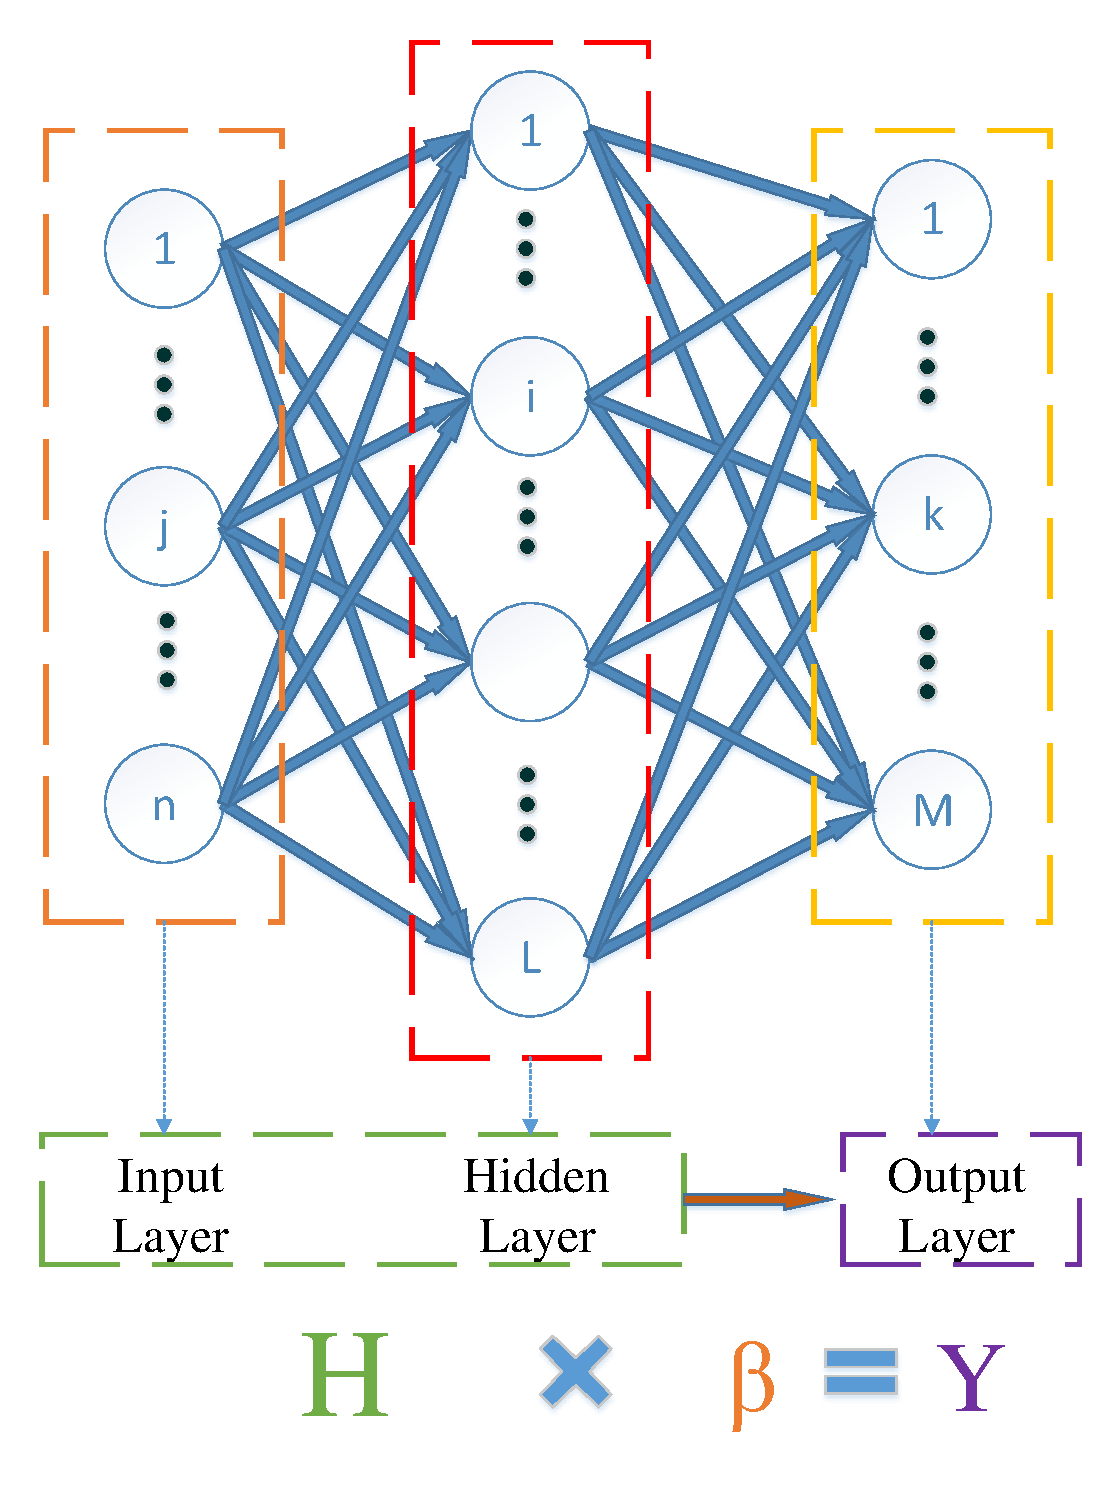
\includegraphics[width=0.6\linewidth]{graphs/ELMs.pdf}
  \caption{The main idea of solving ELMs. The parameters values can be generated randomly. And H can be computed Immediately. Then we can treat the first two layers as H and ELM changes to a simple linear regression form. The parameters $\beta$ between hidden layer and the output layer can be easily and quickly solved.}\label{fig:elms}
\end{figure}

%------------------------------------Propose Method---------------------------------
\section{Proposed Method}
The core idea of the proposed method is that the feature space is divided into many subspaces, and a certain mapping model is learned for each of the subspace. At this point, all the mapping models form the piecewise non-linear SR system. The proposed method mainly includes two parts: the training phase for piecewise non-linear mapping models and the SR reconstruction phase.


\subsection{Piecewise non-linear mapping model}
We extract LR-HR image patch pairs as the training data. The proposed method employs a coarse-to-fine strategy to classify training data. When the partition is complete, for each subspace, we use the training data arriving here to learn a mapping model. We divide the training data into many subspaces, simultaneously an SR decision tree is constructed. The number of the subspaces equals to the number of leaf nodes. Each leaf node is corresponding to a mapping model. In the SR reconstruction phase, the proposed method searches the appropriate mapping model for each input LR image patch. Fig.~\ref{fig:FlowchartForTrain}is the flowchart of the training phase.

\begin{figure}[htbp]
  \centering
  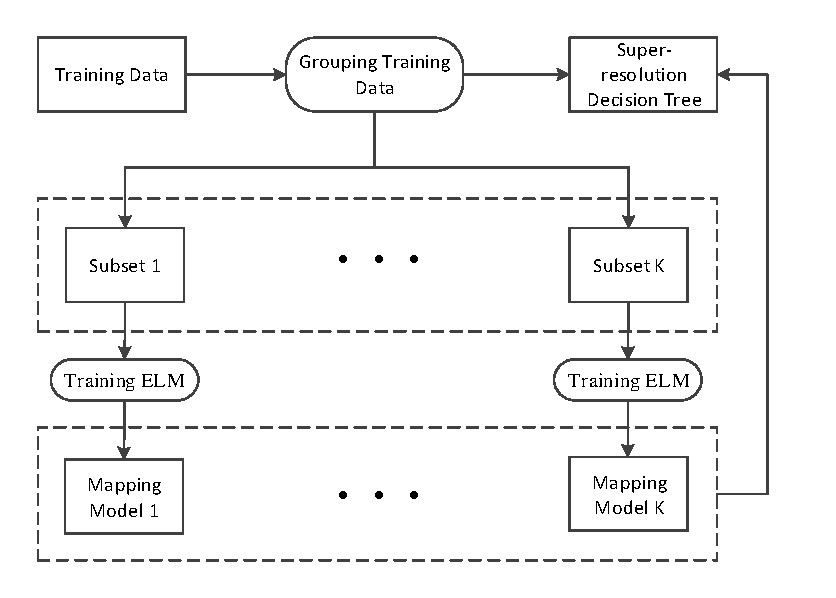
\includegraphics[width=0.8\linewidth]{graphs/FlowForTraining_e.pdf}
  \caption{Flowchart outlining the training phase}\label{fig:FlowchartForTrain}
\end{figure}

The selection of image features and algorithm of the decision tree will affect the running speed and the SR reconstruction result. Luo et al \cite{LUO2018315} proposed method performs the Hadamard transform on LR image patches to extract their image features (Hadamard pattern). The Hadamard transform only involves in addition and subtraction, which makes the transformation simple and fast. Then, the algorithm select two threshold values and divide patches into three parts, according to the results of the generated Hadamard patterns. This is the rule of dividing tree nodes. Each leaf node of the decision is corresponding to a set of training data. Then, we compute the mapping model using ELM for each leaf node.Non-leaf nodes in the SR decision tree stores the threshold values and the indices that point to its child nodes. Each leaf node stores the index that points to the corresponding mapping model.
Small LR image patches contain little information, while large ones cause much more parameters and over-fitting. The optional side length of the LR image patches is $2\times2$, $4\times4$, $8\times8$, $16\times16$, and $32\times32$ and so on. The order of the corresponding Hadamard matrix is 4, 16, 64, 256, and 1024 and so on. Thus, we set the size of the LR image patch to $4×4$, and we adopt a Hadamard matrix of 16-order as \cite{LUO2018315}. The first column of $Q_{16}$ is all ones, and we delete it. The reduced Hadamard matrix is $Q_{15}$. Later, the so called Hadamard matrix is $Q_{15}$.

Each mapping model consists of three parts as mentioned above: the randomly generated input coefficient matrix and hidden layer bias, and the output coefficient matrix that is calculated mathematically. We use ELM to compute the mapping model. The LR training data are the inputs of the single-hidden-layer feed-forward neural network and the HR training data are the targets. First, a randomly generated coefficient matrix maps the LR training data to the hidden layer. Then, the randomly mapped results are add the randomly generated hidden layer bias. The sum is processed by the activation function, and it is the output of the hidden layer. Last, the output coefficient matrix is calculated using the output of the hidden layer and the target values.
For the leaf node q, $H_q$ represents its HR training data, and $L_q$ denotes its LR training data. $L_q$ and $H_q$ are matrix that are stacked by multiple vectorized LR patches and HR patches respectively. The calculation of the mapping model are formulated as
\begin{equation}\label{eq:map_model_1}
  H^*=w_q L_q+b_q
\end{equation}
\begin{equation}\label{eq:map_model_2}
  H=G(H^*)
\end{equation}
Where $w_q$ is the randomly generated input coefficient matrix, $b_q$ represents the randomly generated hidden layer bias. $H^*$ denotes the input of the hidden layer. $G(\bullet)$ is the activation function, and a sigmoid function is adopted in our method. $H$ represents the output matrix of the hidden layer

$\beta_q$ is the output coefficient matrix that connects the hidden layer and the output layer. We can get it by Eq.~\ref{eq:SoluB}. For the leaf node q, its mapping models consists of $w_q$, $b_q$, and$\beta_q$.
The proposed method constructs an SR decision tree. Each leaf node is corresponding to a non-linear mapping model that describes the mapping relationship between the LR space to HR space. Our method addresses the single-image SR problem at patch level. For each LR image patch, there is only one mapping model corresponds to it. We don’t need to preprocess the input LR image using basic interpolation algorithm. It effectively reduces computations and the smoothness in the output HR image.

\subsection{SR reconstruction scheme}
We first extract LR image patches from the input LR image, then, we perform the Hadamard transform on them to compute their Hadamard patterns. The generated Hadamard patterns are the bases of searching their corresponding mapping models. Their Hadamard patterns are compared with the threshold values in the SR decision tree, then, these LR image patches are passed to their corresponding leaf nodes and mapped to the HR space. All the predicted HR patches form the target output. In the searching process of mapping models, a ternary search algorithm is employed. All the generated HR patches form the output HR image. Fig.~\ref{fig:FlowForRecon} is flowchart of the SR reconstruction.
\begin{figure}[htbp]
  \centering
  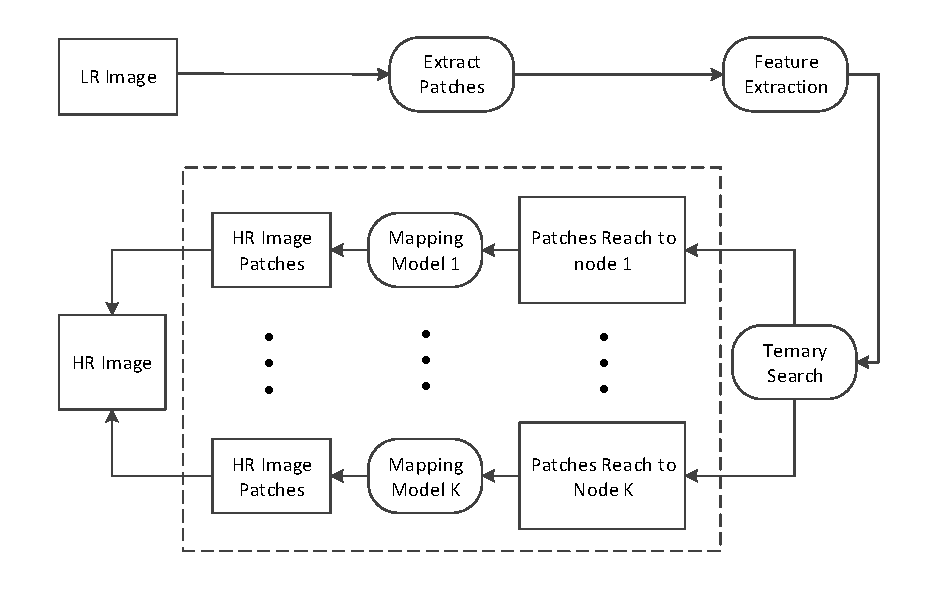
\includegraphics[width=0.8\linewidth]{graphs/FlowForRecon_e.pdf}
  \caption{Flowchart outlining the SR reconstruction phase}\label{fig:FlowForRecon}
\end{figure}



\section{Experimental Results}
The training dataset in our method contains 91 natural images \cite{yang2010image} . We use \cite{LUO2018315} as our decision tree ,which employs a ternary searching algorithm. The size of the LR training image patch is set to 4×4, and the size of the corresponding HR training image patch is set to $s×s$ (s is the upscaling factor). In the SR reconstruction phase, when the upscaling factor is 2, the size of the generated HR image patch is 2×2. No matter in the training phase or the reconstruction phase, the extracted LR image patches have overlapping regions, and the generated HR image patches have no overlapping regions as \cite{LUO2018315}. The minimum size of each leaf node’s training samples is set to 512, and the parameter v of the decision tree is set to 0.5 ,which is same to \cite{LUO2018315}. In the proposed method , the YCrCb color space is used. The SR reconstruction is only performed on luminance channel. Human is more sensitive to high-frequency brightness changes than high-frequency color changes. Thus, many other SR methods employ the same settings. To generate RGB color images, the proposed method first changes the RGB color space to YCrCb color space, then it performs the SR reconstruction on the luminance channel. The chromatic channels are upscaled by the bicubic interpolation algorithm. Last, our method changes the YCrCb color space to RGB color space to generate the HR output.
\subsection{Experiment on images blurred by Gaussian filter}
To verify the effectiveness of the proposed method, we compared it with other SR methods in image quality (i.e., PSNR and SSIM) and running time. The ANR method\cite{timofte2013anchored}, the A+ method \cite{timofte2014a+}, the SRHDT$\_$f* method \cite{huang2017learning}, the RFL method \cite{schulter2015fast}, the SRCNN method \cite{dong2016image}, and the LapSRN method \cite{lai2017deep} are used for comparison. We use their published implementations. The upscaling factor is set to 2. We use the configuration recommended by the respective author. Our computing platform was an Intel Core i7-4790 CPU 3.60 GHZ 4 core processor with 16GB RAM.
\subsubsection{Experimental Setting}

In this experiment, to imitate the real imaging process, all the images in testing image datasets Set5 and Set14 were first blurred by a Gaussian filter and then down-sampled by bicubic interpolation with a scaling factor of two to generate the corresponding LR testing images. The size of the Gaussian filter is 5$\times$5, and the standard deviation is 1.6.
The pre-trained mapping models, testing images, and the testing codes can be downloaded at this URL: https://github.com/youyouyimu/ELMbSISR.

\subsubsection{The Number of Hidden Nodes}
In the proposed method, the number of hidden nodes is have a great effect on SR reconstruction performance. ELM is not sensitive to the number of hidden nodes \cite{huang2012extreme}. However, an appropriate number of hidden nodes can achieve better accuracy. Our method is intended to reconstruct the HR image with high quality from the LR image. To determine the optimal number of hidden nodes, we have conducted an experiment. The results are shown in Fig.~\ref{fig:hiddeNodes}. Obviously, when the number of hidden nodes increases from 10 to 30, the improvement of the average PSNR on Set5 is 1.1dB. When the number of hidden nodes is bigger than 40, the average PSNR on Set5 gradually decreases. Moreover, the bigger the number of hidden nodes, the longer the training time. We have to compute more parameters. Thus, in the proposed method, we set the number of hidden nodes to 35.

\begin{figure}[htbp]
  \centering
  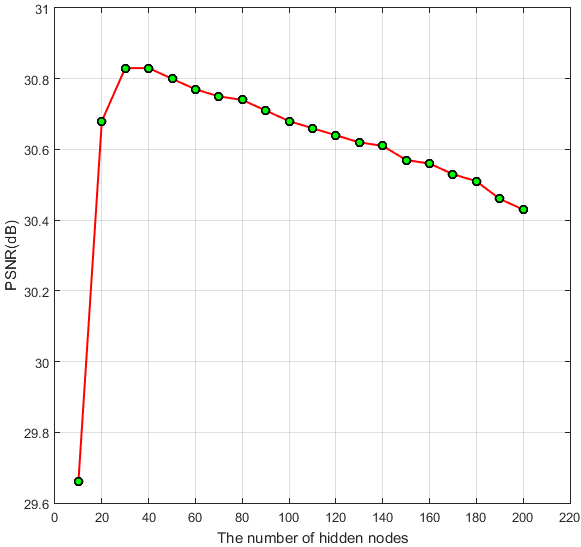
\includegraphics[width=0.6\linewidth]{Fig_hiddenNodes.png}
  \caption{Upscaling factor is two. The relationship between the average PSNR on Set5 and the number of hidden nodes.}\label{fig:hiddeNodes}
\end{figure}

\subsubsection{Experimental Analysis}

As can be observed in Fig.~\ref{fig:compares_1} and Table\ref{tab:result_avg}, in comparison with the ANR method\cite{timofte2013anchored}, the A+ method\cite{timofte2014a+} [31], the SRHDT$\_$f* method\cite{huang2017learning} [46], the RFL method\cite{schulter2015fast}, the SRCNN method\cite{dong2016image}, the LapSRN method\cite{lai2017deep}, and PLHT method(Piecewise linear regression-based single image super-resolution via Hadamard transform)\cite{LUO2018315}, our proposed method achieves the highest average PSNR with the fast running speed. Our method better balances the reconstruction accuracy and the running time. The upscaling factor is two. Figure \ref{fig:barchart1} shows the normalized average PSNR, SSIM, and running time on Set5. Table \ref{tab:result_PSNR_1_Set14_all}, \ref{tab:result_SSIM_1_Set14_all}, and \ref{tab:Time_set14_1_all} shows the PSNR, SSIM, and running time by different methods on Set14.

\begin{figure}[htbp]
\centering
        \subfigure[]{
            \begin{minipage}[b]{0.48\textwidth}
                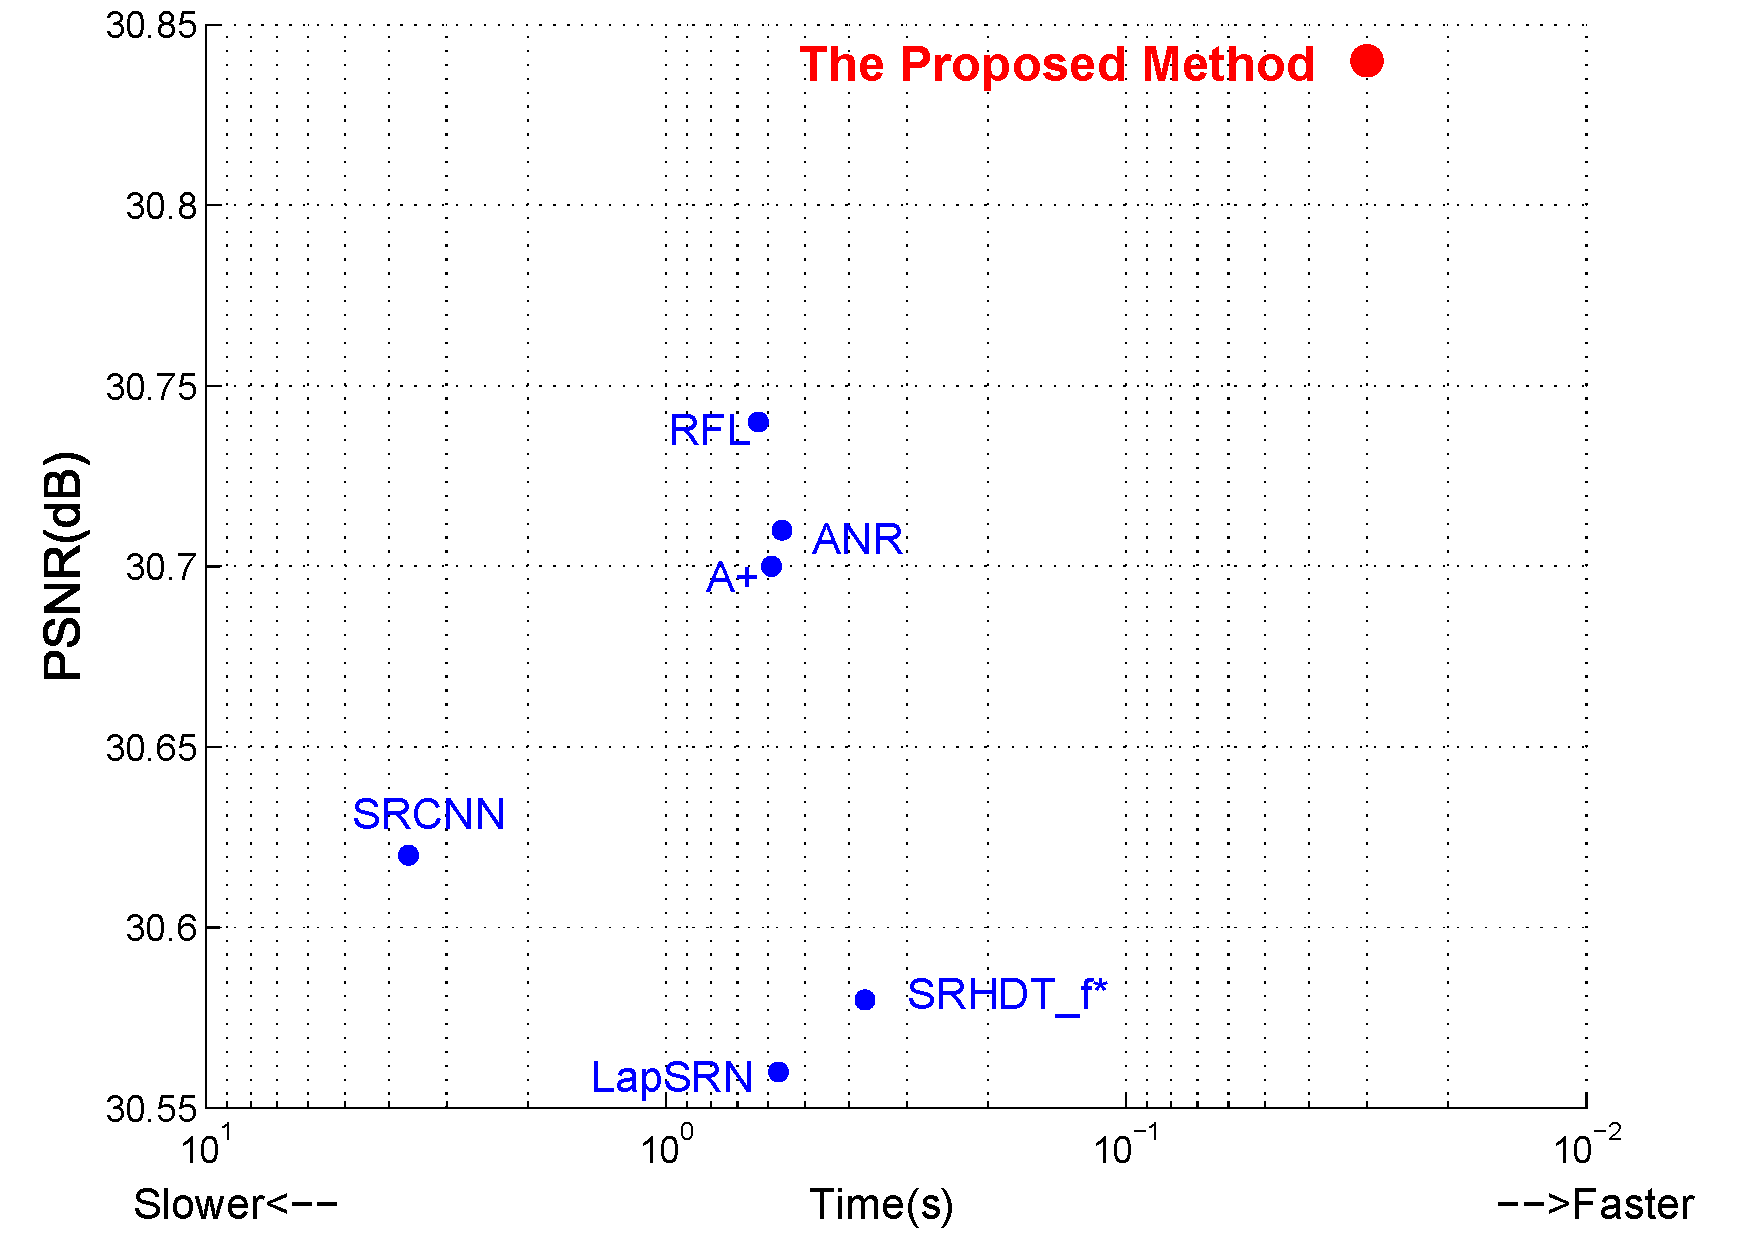
\includegraphics[width=1\textwidth]{chart_set5.pdf}

            \end{minipage}
           }
        \subfigure[]{
            \begin{minipage}[b]{0.48\textwidth}
                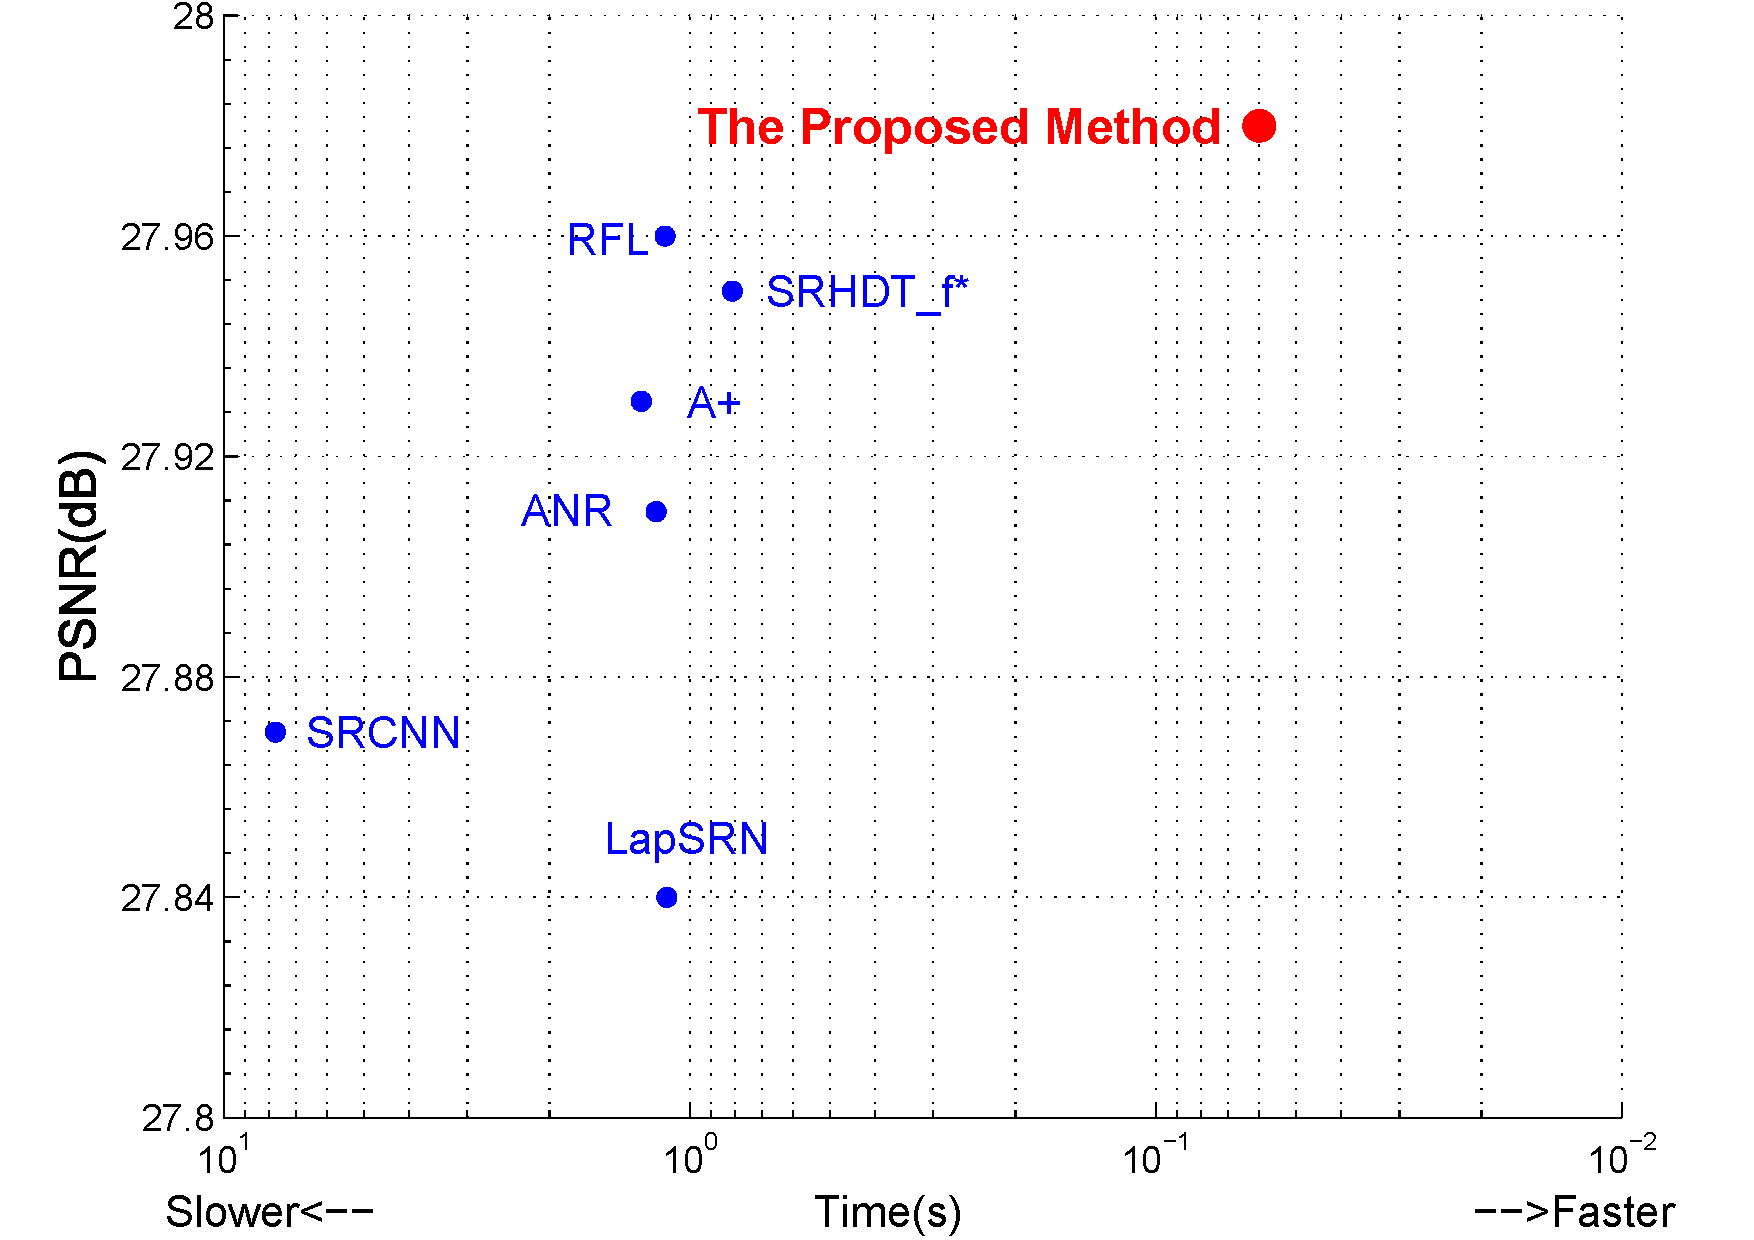
\includegraphics[width=1\textwidth]{chart_set14.pdf}

            \end{minipage}
        } \\

\caption{Trade-off between the accuracy and the running speed. The upscaling factor is two. (a) and (b) show the trade-off between the average PSNR and the running time. The proposed method is the best.}
\label{fig:compares_1}
\end{figure}
We divide the comparison methods into three parts:sparse-coding based methods (ANR and A+),decision tree based methods(SRHDT$\_$f*, RFL and PLHT) and convolutional neural network based methods(SRCNN and LapSRN). Firstly, The sparse-coding based methods always need a long time to find the solution. Secondly, The SRHDT$\_$f* method is a decision-tree-based SR method, and the RFL method is random-forest based. The RFL method constructs a SR random forest, and the number of the decision tree is much more than the proposed method. Both the SRHDT$\_$f*method and RFL method have to spend more time to searching the mapping models. PLHT use same a decision tree as ours,but linear functions in PLHT loss some abilities in mapping. The comparison results show that the proposed method obtains a better trade-off between the reconstruction accuracy and the running time.

% Results on set5 and set14
\begin{table}[]
\centering
\caption{Upscaling factor is two. The average PSNR, SSIM, and running time obtained by different methods on Set5 and Set14. The {\color{red} red} font indicates that the corresponding item ranks first, and the {\color{blue} blue} font indicates that the corresponding item ranks second. The proposed method balances the accuracy and the running time better.}
\label{tab:result_avg}
\resizebox{\textwidth}{!}{
\begin{tabular}{@{}lllllllllll@{}}
\toprule
                                             &                              &\multicolumn{9}{c}{Methods}                                                                              \\ \cmidrule(l){3-11}
\multirow{-2}{*}{Dataset}                    & \multirow{-2}{*}{Measures}   & Bicubic & ANR    & A+                           & SRHDT\_f*                   & RFL                           & SRCNN  & LapSRN        &PLHT               & OUR                           \\ \midrule
\multicolumn{1}{l|}{}                        & PSNR                         & 29.96   & 30.71  & 30.7                         & 30.58                       & {\color[HTML]{3531FF} 30.74}  & 30.62  & 30.56     &{\color[HTML]{FE0000} 30.89}                  & {\color[HTML]{FE0000} 30.89}  \\
\multicolumn{1}{l|}{}                        & SSIM                         & 0.8615  & 0.8797 & 0.8810 & 0.8793              & 0.8805                      & 0.8783 
        & 0.8804 & {\color[HTML]{3531FF} 0.8825}                            & {\color[HTML]{3531FF} 0.8819} \\
\multicolumn{1}{l|}{\multirow{-3}{*}{Set5}}  & TIME(s)                      & 0       & 0.56   & 0.59                         & 0.37                        & 0.63                          & 3.63   & 0.57    &{\color[HTML]{FE0000} 0.02}                             & {\color[HTML]{3531FF} 0.03}   \\ \midrule
\multicolumn{1}{l|}{}                        & PSNR                         & 27.3    & 27.91  & 27.93                        & 27.95                       &  27.96 
& 27.87  & 27.84                             &{\color[HTML]{3531FF}27.99 }  & {\color[HTML]{FE0000} 28.02}  \\
\multicolumn{1}{l|}{}                        & SSIM                         & 0.7673  & 0.7913 & {\color[HTML]{FE0000} 0.793} & 0.79                        & {\color[HTML]{3531FF} 0.7919} & 0.7909 & {\color[HTML]{FE0000} 0.793} &0.7913 & 0.7903                       \\
\multicolumn{1}{l|}{\multirow{-3}{*}{Set14}} & TIME(s)                      & 0       & 1.18   & 1.27                         &  0.81                        & 1.13                          & 7.74   & 1.12          &{\color[HTML]{FE0000} 0.03}               & {\color[HTML]{3531FF} 0.06} \\ \bottomrule
\end{tabular}}
\end{table}


% PSNR on set 14 for all images
% \usepackage{booktabs}
\begin{table}[]
\centering
%\captionsetup{singlelinecheck = false,font={bf},skip=0pt}
\caption{Upscaling factor is two. The PSNR obtained by different methods on Set14. \textbf{Bold} font indicates that the corresponding item ranks first.}
\label{tab:result_PSNR_1_Set14_all}
\resizebox{\textwidth}{!}{
\begin{tabular}{@{}ccccccccc@{}}
\toprule
                                & \multicolumn{8}{c}{Methods}                                               \\ \cmidrule(l){2-9}
%Images                          & \multicolumn{8}{c}{Methods}                                                                                           \\ \cmidrule(l){2-9}
\multirow{-2}{*}{Images}        & Bicubic & ANR            & A+             & SRHDT\_f*      & RFL   & SRCNN          & LapSRN         & OUR            \\ \midrule
\multicolumn{1}{c|}{Baboon}     & 23.17   & 23.47          & \textbf{23.48} & \textbf{23.48} & 23.47 & \textbf{23.48} & \textbf{23.48} & 23.44          \\
\multicolumn{1}{c|}{Barbara}    & 26.11   & 26.46          & \textbf{26.47} & \textbf{26.47} & 26.45 & 26.46          & 26.44          & 26.4           \\
\multicolumn{1}{c|}{Bridge}     & 24.27   & 24.74          & 24.77          & \textbf{24.79} & 24.78 & 24.77          & 24.74          & \textbf{24.79} \\
\multicolumn{1}{c|}{Coastguard} & 26.49   & 27.04          & \textbf{27.08} & 27.04          & 27.05 & 27.04          & 27.06          & \textbf{27.08}          \\
\multicolumn{1}{c|}{Comic}      & 23      & 23.59          & 23.6           & \textbf{23.67} & 23.59 & 23.57          & 23.56          & 23.50          \\
\multicolumn{1}{c|}{Face}       & 32.65   & 33.1           & \textbf{33.11} & 33.02          & 33.04 & 33.06          & \textbf{33.11} & 32.99          \\
\multicolumn{1}{c|}{Flowers}    & 27.04   & 27.71          & 27.73          & \textbf{27.78} & 27.7  & 27.68          & 27.63          & 27.67          \\
\multicolumn{1}{c|}{Foreman}    & 30.25   & 31.3           & 31.33          & 31.38          & 31.59 & 31.17          & 31.21          & \textbf{32.26} \\
\multicolumn{1}{c|}{Lenna}      & 31.33   & 32.01          & 32             & 31.98          & 31.99 & 31.92          & 31.92          & \textbf{32.02}            \\
\multicolumn{1}{c|}{Man}        & 26.87   & 27.38          & 27.4           & \textbf{27.41} & 27.39 & 27.35          & 27.32          & 27.37         \\
\multicolumn{1}{c|}{Monarch}    & 29.07   & 29.87          & 29.9           & 29.97          & 29.95 & 29.81          & 29.71          & \textbf{30.03} \\
\multicolumn{1}{c|}{Pepper}     & 31.95   & 32.66          & 32.7           & 32.7           & 32.79 & 32.54          & 32.53          & \textbf{32.91} \\
\multicolumn{1}{c|}{PPT3}       & 23.64   & 24.36          & 24.43          & 24.52          & 24.51 & 24.32          & 24.2           & \textbf{24.55}          \\
\multicolumn{1}{c|}{Zebra}      & 26.15   & 27.07          & 27.06          & 27.08          & 27.09 & 26.96          & 26.89          & \textbf{27.19} \\
\multicolumn{1}{c|}{Average}    & 27.3    & 27.91          & 27.93          & 27.95          & 27.96 & 27.87          & 27.84          & \textbf{28.02} \\ \bottomrule
\end{tabular}}
\end{table}

% SSIM on set14 for all image
% \usepackage{booktabs}
\begin{table}[]
\centering
%\captionsetup{singlelinecheck = false,font={bf},skip=0pt}
\caption{Upscaling factor is two. The SSIM obtained by different methods on Set14. \textbf{Bold} font indicates that the corresponding item ranks first.}
\label{tab:result_SSIM_1_Set14_all}
\resizebox{\textwidth}{!}{
\begin{tabular}{@{}ccccccccc@{}}
\toprule
                                & \multicolumn{8}{c}{Methods}                                               \\ \cmidrule(l){2-9}
%Images                          & \multicolumn{8}{c}{Methods}                                                                                         \\ \cmidrule(l){2-9}
\multirow{-2}{*}{Images}        & Bicubic & ANR    & A+              & SRHDT\_f*       & RFL             & SRCNN  & LapSRN          & OUR             \\ \midrule
\multicolumn{1}{c|}{Baboon}     & 0.5299  & 0.5624 & 0.5628          & 0.5625          & 0.5618          & 0.5626 & \textbf{0.5639} & 0.5617          \\
\multicolumn{1}{c|}{Barbara}    & 0.7485  & 0.7691 & \textbf{0.7698} & 0.7637          & 0.7679          & 0.7687 & 0.7695          & 0.7660          \\
\multicolumn{1}{c|}{Bridge}     & 0.6322  & 0.6685 & 0.6695          & \textbf{0.6713} & 0.6678          & 0.6700 & 0.6699          & 0.6676         \\
\multicolumn{1}{c|}{Coastguard} & 0.6180  & 0.6557 & 0.6581          & 0.6398          & 0.6523          & 0.6566 & \textbf{0.6596} & 0.6394         \\
\multicolumn{1}{c|}{Comic}      & 0.6943  & 0.7335 & \textbf{0.7356} & 0.7335          & 0.7342          & 0.7314 & 0.7343          & 0.7276          \\
\multicolumn{1}{c|}{Face}       & 0.7920  & 0.8063 & 0.8071          & 0.8033          & 0.8073          & 0.8088 & \textbf{0.8115} & 0.8068         \\
\multicolumn{1}{c|}{Flowers}    & 0.7994  & 0.8246 & \textbf{0.8257} & 0.8221          & 0.8253          & 0.8235 & 0.8252          & 0.8214          \\
\multicolumn{1}{c|}{Foreman}    & 0.8921  & 0.9071 & 0.9096          & 0.9127          & 0.9099          & 0.9051 & 0.9093          & \textbf{0.9143} \\
\multicolumn{1}{c|}{Lenna}      & 0.8531  & 0.8671 & 0.8685          & 0.8639          & 0.8667          & 0.8654 & \textbf{0.8686} & 0.8666         \\
\multicolumn{1}{c|}{Man}        & 0.7429  & 0.7671 & \textbf{0.7678} & 0.7644          & 0.7661          & 0.7667 & 0.7674          & 0.7655          \\
\multicolumn{1}{c|}{Monarch}    & 0.9174  & 0.9294 & 0.9309          & 0.9291          & 0.9298          & 0.9277 & \textbf{0.9304} & \textbf{0.9309} \\
\multicolumn{1}{c|}{Pepper}     & 0.8629  & 0.8741 & 0.8763          & 0.8744          & 0.8764          & 0.8728 & 0.8765          & \textbf{0.8775} \\
\multicolumn{1}{c|}{PPT3}       & 0.8772  & 0.8994 & 0.9058          & 0.9055          & \textbf{0.9066} & 0.9012 & 0.9019          & 0.9059          \\
\multicolumn{1}{c|}{Zebra}      & 0.7812  & 0.8140 & 0.8150          & 0.8133          & \textbf{0.8151} & 0.8125 & 0.8146          & 0.8136          \\
\multicolumn{1}{c|}{Average}    & 0.7673  & 0.7913 & \textbf{0.7930} & 0.7900          & 0.7919          & 0.7909 & \textbf{0.7930} & 0.7903 \\ \bottomrule
\end{tabular}}
\end{table}

% Running time on Set14
% \usepackage{booktabs}
\begin{table}[]
\centering
\caption{Upscaling factor is two. The running time obtained by different methods on Set14. \textbf{Bold} font indicates that the corresponding item ranks first. The running time of the Bicubic method is the baseline, which is not used for comparison.}
\label{tab:Time_set14_1_all}
\resizebox{\textwidth}{!}{
\begin{tabular}{@{}ccccccccc@{}}
\toprule
                                & \multicolumn{8}{c}{Methods}                                               \\ \cmidrule(l){2-9}
\multirow{-2}{*}{Images}        & Bicubic & ANR  & A+   & SRHDT\_f* & RFL  & SRCNN & LapSRN & OUR           \\ \midrule
\multicolumn{1}{c|}{Baboon}     & 0       & 1.11 & 1.20 & 1.13      & 1.24 & 8.14  & 1.10   & \textbf{0.07} \\
\multicolumn{1}{c|}{Barbara}    & 0       & 1.86 & 2.03 & 1.29      & 1.93 & 14.53 & 2.00   & \textbf{0.12} \\
\multicolumn{1}{c|}{Bridge}     & 0       & 1.18 & 1.32 & 1.38      & 1.35 & 9.06  & 1.25   & \textbf{0.07} \\
\multicolumn{1}{c|}{Coastguard} & 0       & 0.51 & 0.55 & 0.37      & 0.56 & 2.41  & 0.51   & \textbf{0.03} \\
\multicolumn{1}{c|}{Comic}      & 0       & 0.46 & 0.49 & 0.47      & 0.55 & 2.43  & 0.58   & \textbf{0.02} \\
\multicolumn{1}{c|}{Face}       & 0       & 0.40 & 0.42 & 0.21      & 0.45 & 1.97  & 0.44   & \textbf{0.02} \\
\multicolumn{1}{c|}{Flowers}    & 0       & 0.93 & 1.00 & 0.76      & 0.94 & 6.16  & 0.91   & \textbf{0.05} \\
\multicolumn{1}{c|}{Foreman}    & 0       & 0.52 & 0.56 & 0.29      & 0.54 & 2.41  & 0.49   & \textbf{0.03} \\
\multicolumn{1}{c|}{Lenna}      & 0       & 1.43 & 1.52 & 0.68      & 1.22 & 9.16  & 1.26   & \textbf{0.07} \\
\multicolumn{1}{c|}{Man}        & 0       & 1.43 & 1.53 & 1.08      & 1.34 & 9.03  & 1.26   & \textbf{0.08} \\
\multicolumn{1}{c|}{Monarch}    & 0       & 2.12 & 2.27 & 1.07      & 1.80 & 13.77 & 1.86   & \textbf{0.11} \\
\multicolumn{1}{c|}{Pepper}     & 0       & 1.43 & 1.51 & 0.66      & 1.24 & 9.08  & 1.26   & \textbf{0.07} \\
\multicolumn{1}{c|}{PPT3}       & 0       & 1.87 & 2.00 & 0.85      & 1.54 & 12.49 & 1.63   & \textbf{0.09} \\
\multicolumn{1}{c|}{Zebra}      & 0       & 1.23 & 1.31 & 1.12      & 1.16 & 7.70  & 1.11   & \textbf{0.06} \\
\multicolumn{1}{c|}{Average}    & 0.      & 1.18 & 1.27 & 0.81      & 1.13 & 7.74  & 1.12   & \textbf{0.06} \\ \bottomrule
\end{tabular}}
\end{table}

\begin{figure}[tb]                   % normalized PSNR, SSIM and running time
\centering
        \subfigure[]{
            \begin{minipage}[b]{0.48\textwidth}
                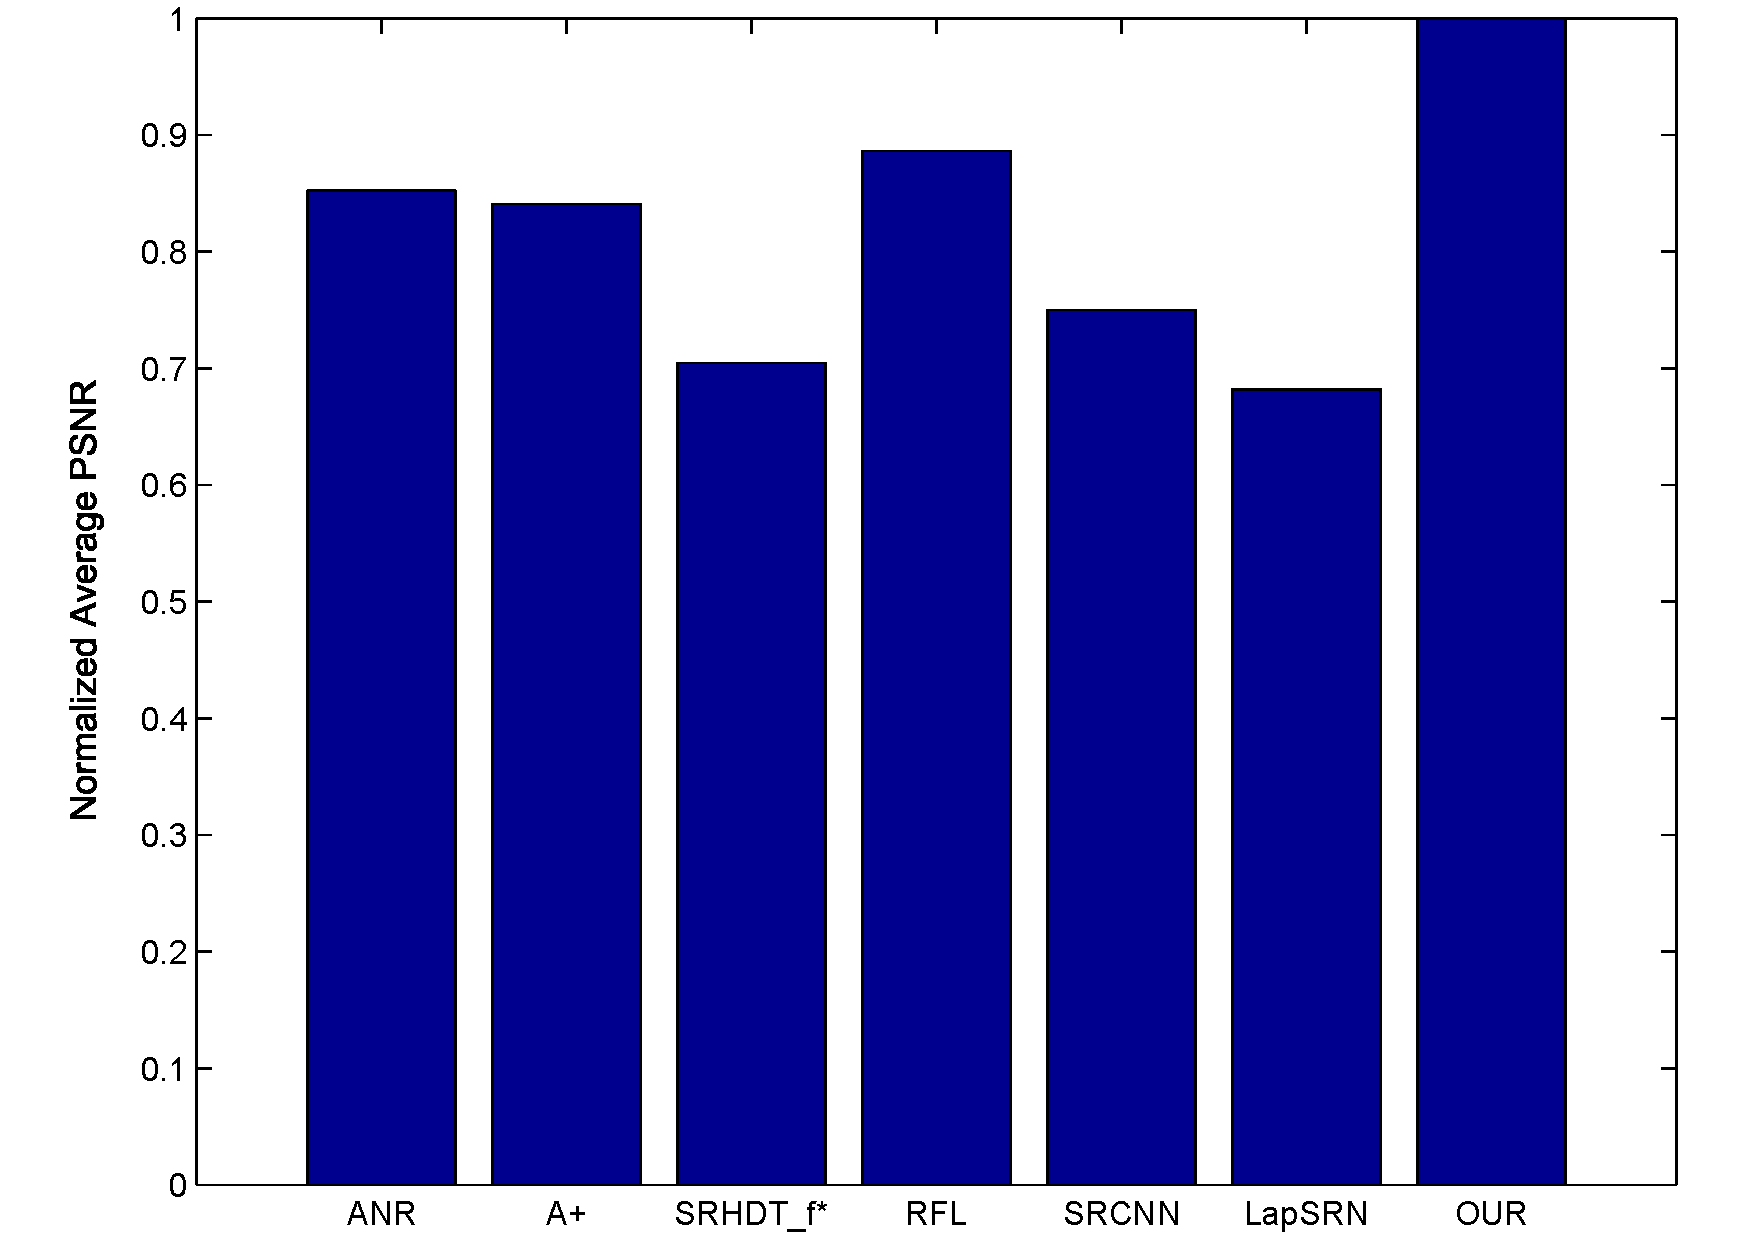
\includegraphics[width=1\textwidth]{norm_PSNR.pdf}
            \end{minipage}
        } \hfill
        \subfigure[]{
            \begin{minipage}[b]{0.48\textwidth}
                \includegraphics[width=1\textwidth]{norm_SSIM.pdf}
            \end{minipage}
        } \\

        \subfigure[]{
            \begin{minipage}[b]{0.49\textwidth}
                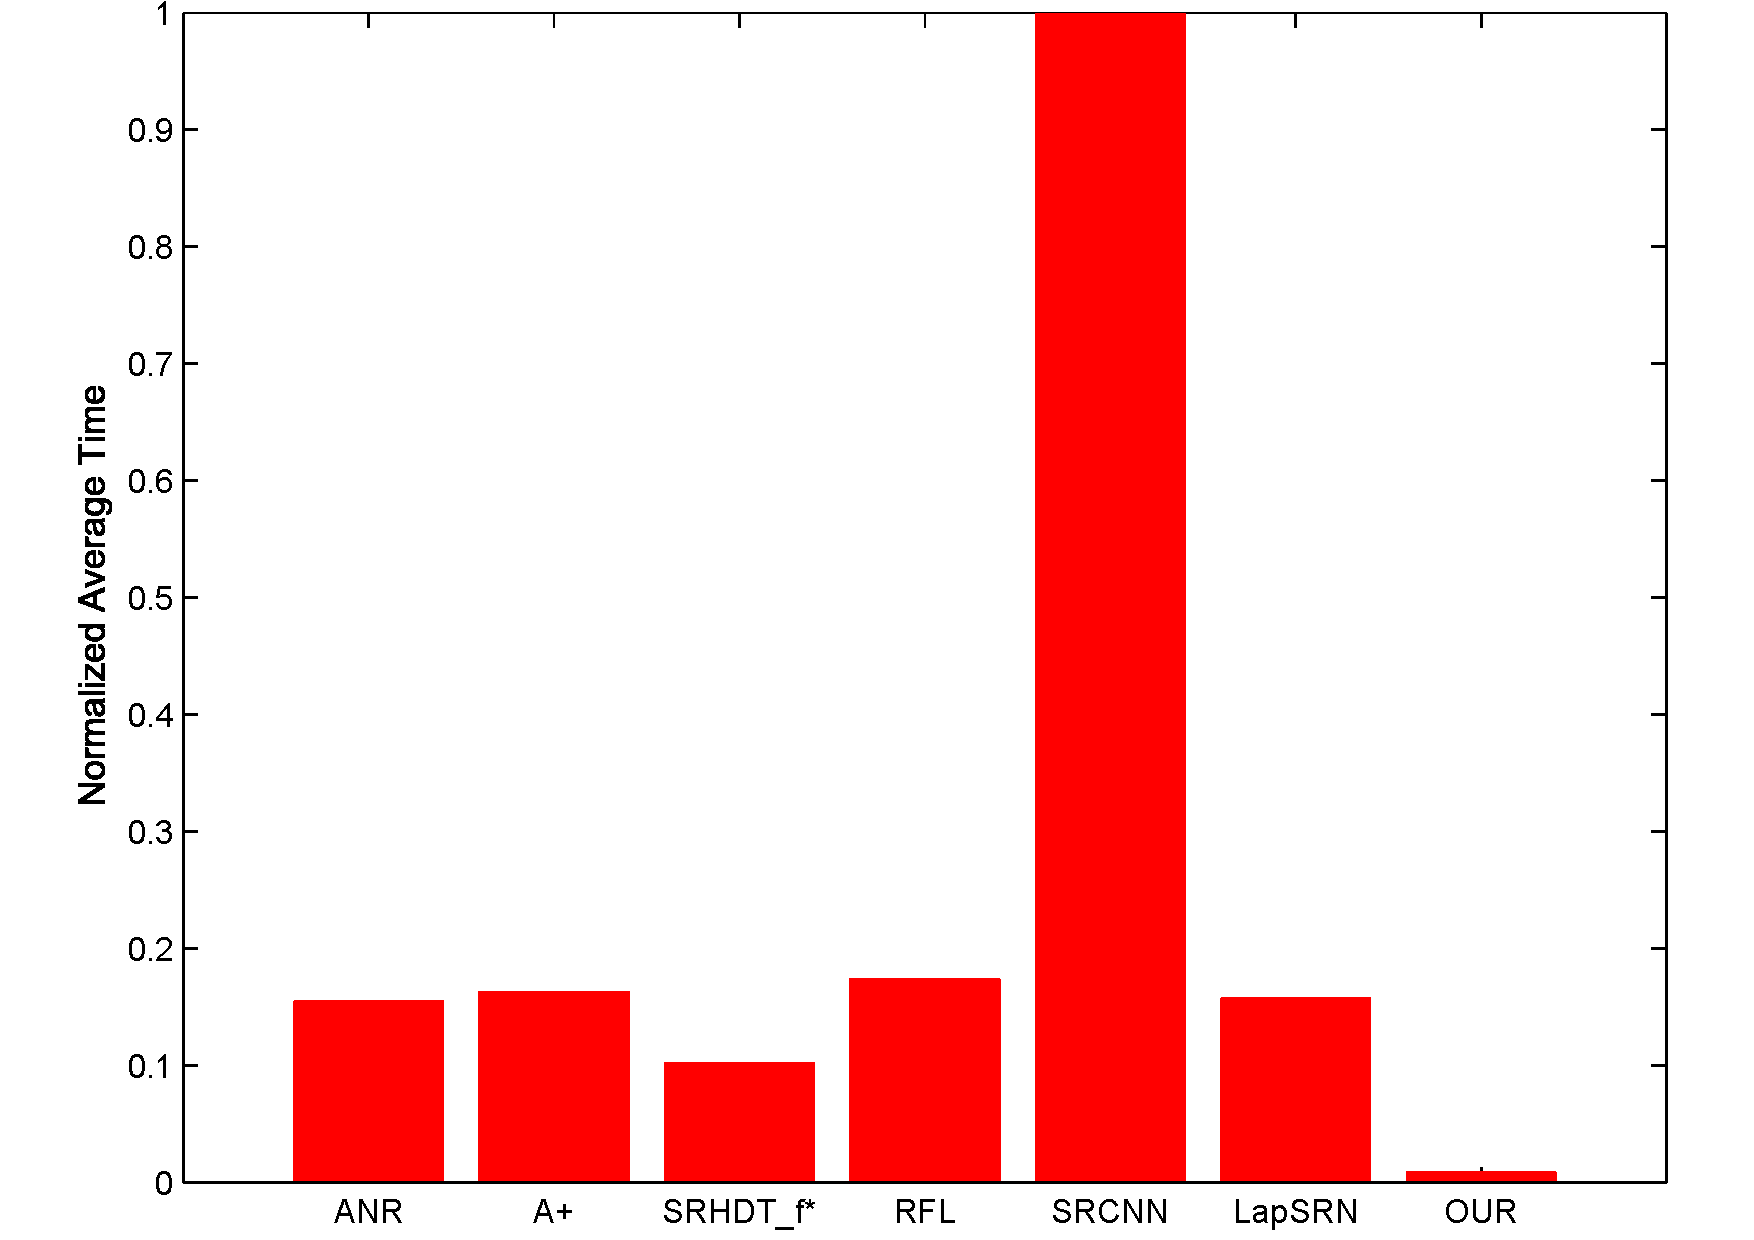
\includegraphics[width=1\textwidth]{norm_time.pdf}
            \end{minipage}
        }
\caption{Normalized average PSNR, SSIM and running time by different methods for a scaling factor of two on Set5.}
\label{fig:barchart1}
\end{figure}

Finally, The SRCNN method and LapSRN method are CNN method. The training dataset of the SRCNN method contains 395909 images, while LapSRN method contains 291 images. However, the proposed method only use 91 natural images for training. As shown in Table.~\ref{tab:result_avg}, our method achieves the higher average PSNR and SSIM than the SRCNN method on Set5 and Set14. Moreover, our method’s running speed is much faster which can be easily found in Figure~\ref{fig:barchart1}.The proposed method employs the Hadamard patterns and ELM. Based on the generated Hadamard patterns, our method divides the feature space into many non-linear subspaces, and it effectively estimates the whole non-linear feature space. Thus, the proposed method obtains the higher reconstruction accuracy. In addition, the use of ELM greatly reduces the training time.

%----------------------------------Experiment 2 ---------------------------------
\subsection{Experiment on images without blurring}
To show our method’s effectiveness, the Bicubic interpolation algorithm is used as a baseline. The SME method\cite{mallat2010super}, the FIRF method \cite{huang2015fast}, and the LapSRN method \cite{lai2017deep} were used for comparison. The computing platform was an Intel Core i7-4790 CPU 3.60 GHZ 4 core processor with 16GB RAM. All the testing codes of other methods were downloaded from the authors’ websites respectively, and all the parameters are set according to the authors’ recommendation.

\begin{table}[]
\centering
\caption{Upscaling factor is two. The average PSNR, SSIM, and running time obtained by different methods on Set5 and Set14. The {\color{red} red} font indicates that the corresponding item ranks first, and the {\color{blue} blue} font indicates that the corresponding item ranks second. The proposed method balances the accuracy and the running time better.}
\label{tab:result_epm2_avg}
\resizebox{0.8\textwidth}{!}{
\begin{tabular}{@{}cccccccc@{}}
\toprule
                                             &                            & \multicolumn{6}{c}{Methods}                                                                                    \\ \cmidrule(l){3-8}
\multirow{-2}{*}{Dataset}                    & \multirow{-2}{*}{Measures} & Bicubic & SME    & FIRF                        & LapSRN                        &PLHT        & OUR                           \\ \midrule
\multicolumn{1}{c|}{}                        & PSNR                       & 33.7    & 33.91  & 33.39                       & {\color[HTML]{FE0000} 37.44}  & 34.9902
 & {\color[HTML]{3531FF} 35.09}  \\
\multicolumn{1}{c|}{}                        & SSIM                       & 0.9304  & 0.9351 & 0.9323                      & {\color[HTML]{FE0000} 0.9590} & 0.9436
& {\color[HTML]{3531FF} 0.9437} \\
\multicolumn{1}{c|}{\multirow{-3}{*}{Set5}}  & TIME(s)                    & 0       & 74.75  & 0.53                        & 0.56                          &{\color[HTML]{FE0000} 0.01}   & {\color[HTML]{3531FF} 0.03}   \\ \midrule
\multicolumn{1}{c|}{}                        & PSNR                       & 30.26   & 30.16  & 29.15                       & {\color[HTML]{FE0000} 32.99}  & 31.28
& {\color[HTML]{3531FF} 31.33}  \\
\multicolumn{1}{c|}{}                        & SSIM                       & 0.8695  & 0.8751 & 0.8674                      & {\color[HTML]{FE0000} 0.9125} & {\color[HTML]{3531FF} 0.8902}   & 0.8892\\
\multicolumn{1}{c|}{\multirow{-3}{*}{Set14}} & TIME(s)                    & 0       & 161.58 & 1.26                        & 1.11                          & {\color[HTML]{FE0000} 0.03}  & {\color[HTML]{3531FF} 0.07} \\ \bottomrule
\end{tabular}}
\end{table}

\subsubsection{Experimental Settings}
Different from Experiment above, this experiment generates testing images in a different way. All the images in Set5\cite{dong2014learning} and Set14\cite{zeyde2010single} are directly downsampled by the bicubic interpolation algorithm, and the upscaling factor is 2. The number of hidden nodes is set to 35. The rest of parameters are same to the last experiment.The pre-trained mapping models, testing images, and the testing codes can be downloaded at this URL: https://github.com/youyouyimu/ELMbSISR.

\begin{figure}[t]                   % the second version of butterfly.png   foreman.png
    \centering
        \subfigure[Bicubic]{
            \begin{minipage}[b]{0.12\textwidth}
                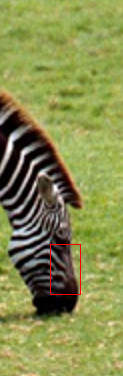
\includegraphics[width=1\textwidth]{compareImage/zebra_crop_Bicu.png} \\
                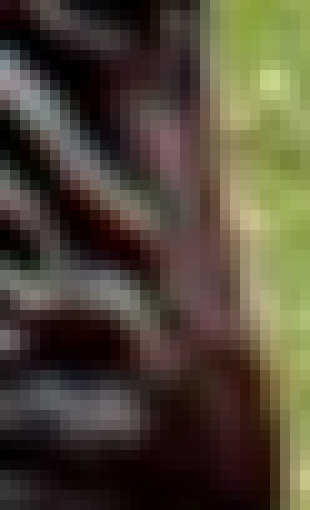
\includegraphics[width=1\textwidth]{compareImage/Bicubic_zebra_mag_2.png}
            \end{minipage}
        }
        \subfigure[SME]{
            \begin{minipage}[b]{0.12\textwidth}
                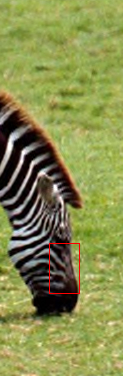
\includegraphics[width=1\textwidth]{compareImage/zebra_crop_SME.png} \\
                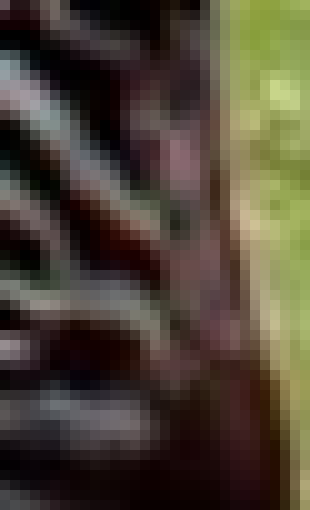
\includegraphics[width=1\textwidth]{compareImage/SME_zebra_mag_2.png}
            \end{minipage}
        }
        \subfigure[LapSRN]{
            \begin{minipage}[b]{0.12\textwidth}
                \includegraphics[width=1\textwidth]{compareImage/zebra_crop_lapSRN.png} \\
                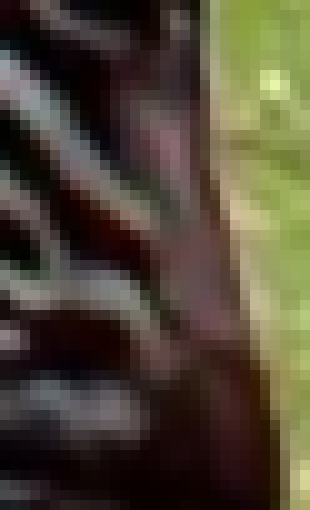
\includegraphics[width=1\textwidth]{compareImage/LapSRN_zebra_mag_2.png}
            \end{minipage}
        }
        \subfigure[PLHT]{
            \begin{minipage}[b]{0.12\textwidth}
                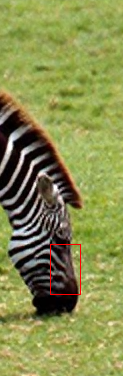
\includegraphics[width=1\textwidth]{compareImage/zebra_crop_PLHT.png} \\
                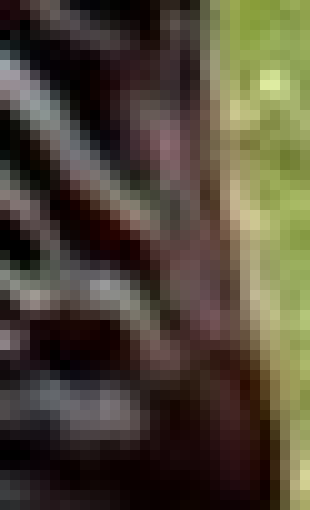
\includegraphics[width=1\textwidth]{compareImage/PLHT_zebra_mag_2.png}
            \end{minipage}
        }
        \subfigure[OUR]{
            \begin{minipage}[b]{0.12\textwidth}
                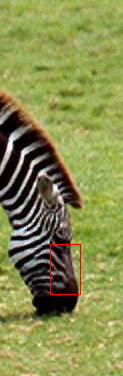
\includegraphics[width=1\textwidth]{compareImage/zebra_crop_OUR.png} \\
                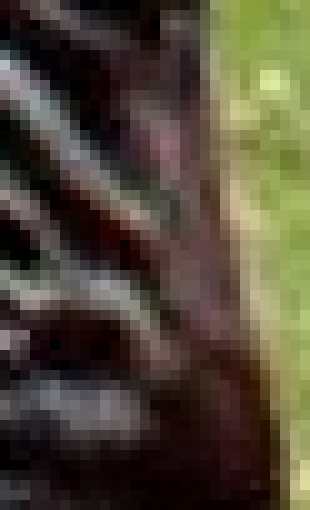
\includegraphics[width=1\textwidth]{compareImage/OUR_zebra_mag_2.png}
            \end{minipage}
        }
        \subfigure[Ori]{
            \begin{minipage}[b]{0.12\textwidth}
                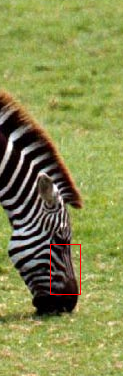
\includegraphics[width=1\textwidth]{compareImage/zebra_crop_ORI.png} \\
                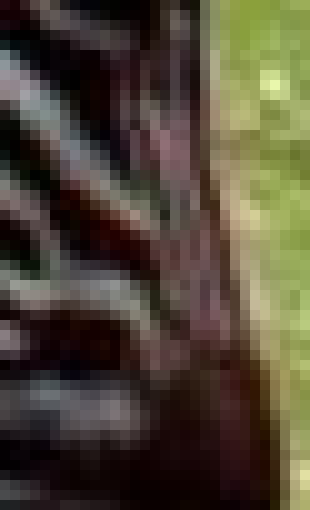
\includegraphics[width=1\textwidth]{compareImage/ORI_zebra_mag_2.png}
            \end{minipage}
        }
    \caption{Comparisons between the Bicubic method, SME method, LapSRN method, and the proposed method. Ori is the original image. The proposed method recover more details, and its reconstructed image is much closer to the original image.}
    \label{fig:color_zebra}
\end{figure}

\begin{figure}[t]
    \centering
        \subfigure[FIRF]{
            \begin{minipage}[b]{0.15\textwidth}
                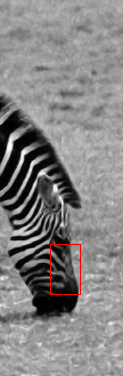
\includegraphics[width=1\textwidth]{compareImage/zebra_crop_FIRF.png} \\
                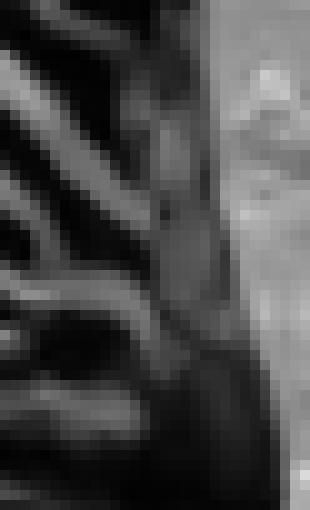
\includegraphics[width=1\textwidth]{compareImage/FIRF_zebra_mag_2.png}
            \end{minipage}
        }
        \subfigure[OUR]{
            \begin{minipage}[b]{0.15\textwidth}
                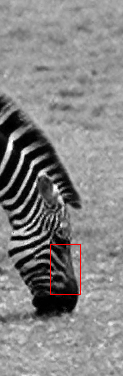
\includegraphics[width=1\textwidth]{compareImage/zebra_crop_G_OUR.png} \\
                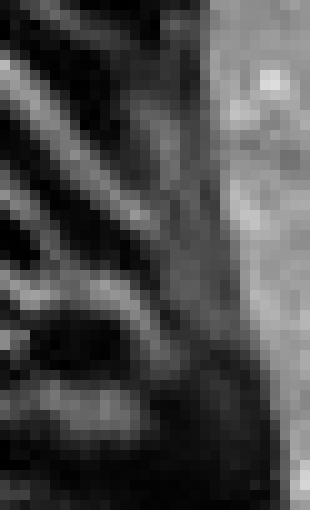
\includegraphics[width=1\textwidth]{compareImage/OUR_zebra_mag_G_2.png}
            \end{minipage}
        }
        \subfigure[Ori]{
            \begin{minipage}[b]{0.15\textwidth}
                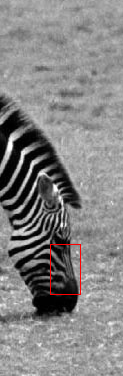
\includegraphics[width=1\textwidth]{compareImage/zebra_crop_G_ORI.png} \\
                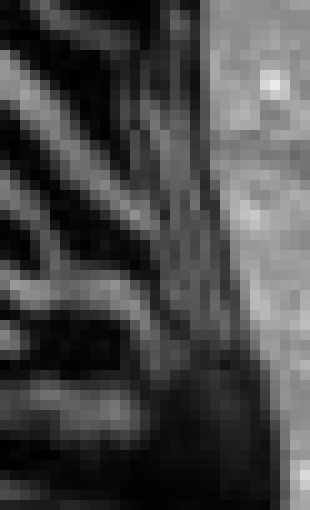
\includegraphics[width=1\textwidth]{compareImage/ORI_zebra_mag_G_2.png}
            \end{minipage}
        }
    \caption{Comparisons between the FIRF method and the proposed method. Ori is the original image. The proposed method recover more details, and its reconstructed image is much closer to the original image.}
    \label{fig:zebra_gray}
\end{figure}

\subsubsection{Experimental Analysis}
Table \ref{tab:result_epm2_avg} shows the objective evaluation for all methods. We treat the bicubic method as the baseline and set its running time to zero. Subsequent analysis of the running speed is based on the comparison of the proposed method with other SR methods. As can be observed in Table \ref{tab:result_epm2_avg}, the proposed method is fastest. The proposed method get the second place on average PSNR and SSIM followed by LapSRN. Our method balances the SR reconstruction accuracy and the running time better. Based on Set5, the average PSNR of our method is 1.27dB higher than that of the FIRF method, and the average SSIM of our method is 0.0067 higher. Moreover, the running speed of our method is much faster, and the speed-up with regard to the FIRF method is 18. Compared with the SME method, the proposed method still obtains the higher average PSNR and SSIM. In addition, the speed-up of running speed is 2491.67. Based on Set14, the proposed method is still competitive in the PSNR and SSIM. The running speed of our method is the fastest. The speed-up with respect to the FIRF method and SME method is 18 and 2308.29 respectively.

Figure \ref{fig:color_zebra}, Figure \ref{fig:zebra_gray}, Figure \ref{fig:flower_color} and Figure \ref{fig:flower_gray} shows the visual comparison of all methods on the image 'zebra' and 'flower'. The FIRF method algorithm only deals with the gray images. Thus, we change the reconstructed images into gray images to perform subjective evaluation, as shown in Figure \ref{fig:zebra_gray} and Figure \ref{fig:flower_gray}. We perform close-up on reconstructed details in the red box.

As shown in Figure \ref{fig:color_zebra}, it is easy to find that the reconstructed results of the Bicubic method, the SME method, and the LapSRN method are too smooth, especially the region below the eyes of this zebra. In the original image, the pixels in white stripes irregularly changes, and there are differences in brightness between them. The proposed method can better reconstruct the texture details in the white stripes, and it can also recover more high-frequency details. Thus, the proposed method is much closer to the original image. In Figure \ref{fig:zebra_gray}, the SR reconstruction result of the FIRF method is too smooth, especially the white stripes and the region above the nose. In comparison with them, the proposed method can recover more texture details (high-frequency details), and its vision quality is better.
\begin{figure}[htbp]
    \centering
        \subfigure[Bicubic]{
            \begin{minipage}[b]{0.12\textwidth}
                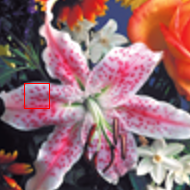
\includegraphics[width=1\textwidth]{compareImage/flower_crop_2_Bicubic.png} \\
                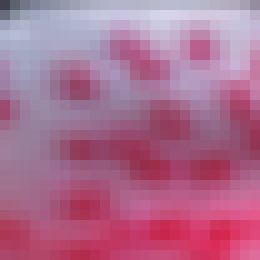
\includegraphics[width=1\textwidth]{compareImage/Bicubic_flowers_mag_2.png}
            \end{minipage}
        }
        \subfigure[SME]{
            \begin{minipage}[b]{0.12\textwidth}
                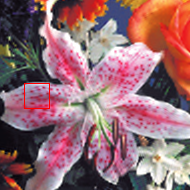
\includegraphics[width=1\textwidth]{compareImage/flower_crop_2_SME.png} \\
                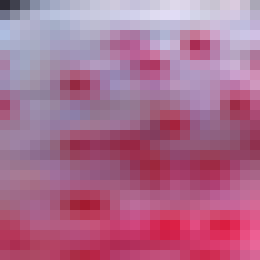
\includegraphics[width=1\textwidth]{compareImage/SME_flowers_mag_2.png}
            \end{minipage}
        }
        \subfigure[LapSRN]{
            \begin{minipage}[b]{0.12\textwidth}
                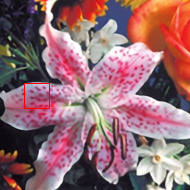
\includegraphics[width=1\textwidth]{compareImage/flower_crop_2_LapSRN.png} \\
                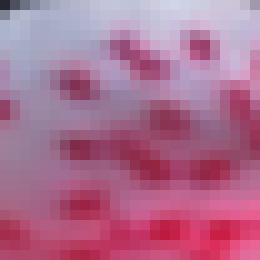
\includegraphics[width=1\textwidth]{compareImage/LapSRN_flowers_mag_2.png}
            \end{minipage}
        }   
        \subfigure[PLHT]{
            \begin{minipage}[b]{0.12\textwidth}
                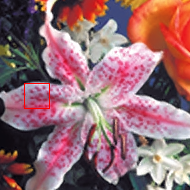
\includegraphics[width=1\textwidth]{compareImage/flower_crop_PLHT.png} \\
                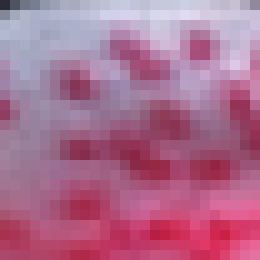
\includegraphics[width=1\textwidth]{compareImage/PLHT_flower_mag_2.png}
            \end{minipage}
        }
        \subfigure[OUR]{
            \begin{minipage}[b]{0.12\textwidth}
                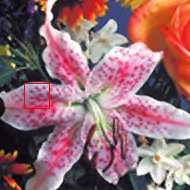
\includegraphics[width=1\textwidth]{compareImage/flower_crop_2_OUR.png} \\
                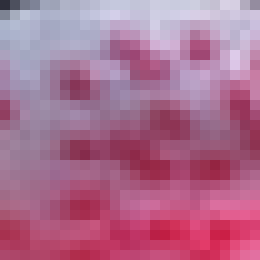
\includegraphics[width=1\textwidth]{compareImage/OUR_flowers_mag_2.png}
            \end{minipage}
        }
        \subfigure[Ori]{
            \begin{minipage}[b]{0.12\textwidth}
                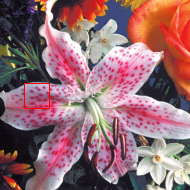
\includegraphics[width=1\textwidth]{compareImage/flower_crop_2_ORI.png} \\
                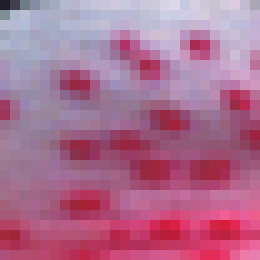
\includegraphics[width=1\textwidth]{compareImage/ORI_flowers_mag_2.png}
            \end{minipage}
        }
    \caption{ Comparisons between the Bicubic,SME,LapSRN PLHT methods and the proposed method. Ori is the original image. The proposed method recover more details, and its reconstructed image is much closer to the original image.}
    \label{fig:flower_color}
\end{figure}

Figure \ref{fig:flower_color}, and Figure \ref{fig:flower_gray} show the reconstructed images of all methods on image 'flower'. The proposed method’s reconstructed image shows that our method can better recover the texture details between the red dots on the petals. As we can see from the original image, the region between the red dots on the petals is not pure white. The texture in the region is complicated. The bicubic method, SME method, LapSRN method, and FIRF method smooth this kind of region, and the original texture does not exist. The proposed method can recover texture details well.

Objectively, the proposed method obtains better evaluation results than the bicubic method, SME method, and FIRF method. Subjectively, our method performs better in recovering high-frequency details, and our reconstructed images are much closer to the original images. The LapSRN method performs best in the objective evaluation. We only test its running time on a CPU platform, and our method achieves a faster running speed. The speed-up on Set5 is 18.67, and that on Set14 is 15.86. The reconstructed images of the LapSRN method involve heavy smoothness. However, the proposed method’s SR reconstructed images contain much more high-frequency details.
\begin{figure}[htbp]
    \centering
        \subfigure[LapSRN]{
            \begin{minipage}[b]{0.17\textwidth}
                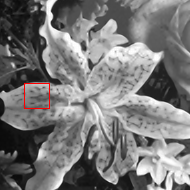
\includegraphics[width=1\textwidth]{compareImage/flower_crop_2_FIRF.png} \\
                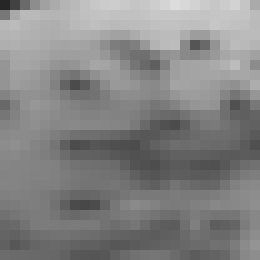
\includegraphics[width=1\textwidth]{compareImage/FIRF_flowers_mag_2.png}
            \end{minipage}
        }
        \subfigure[OUR]{
            \begin{minipage}[b]{0.17\textwidth}
                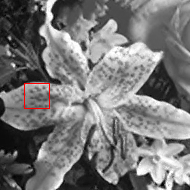
\includegraphics[width=1\textwidth]{compareImage/flower_crop_G_2_OUR.png} \\
                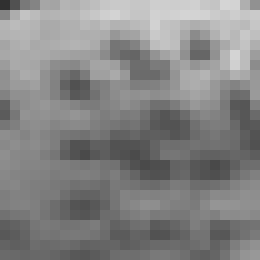
\includegraphics[width=1\textwidth]{compareImage/OUR_flowers_mag_G_2.png}
            \end{minipage}
        }
        \subfigure[Ori]{
            \begin{minipage}[b]{0.17\textwidth}
                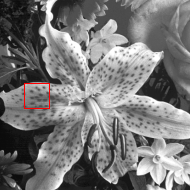
\includegraphics[width=1\textwidth]{compareImage/flower_crop_G_2_ORI.png} \\
                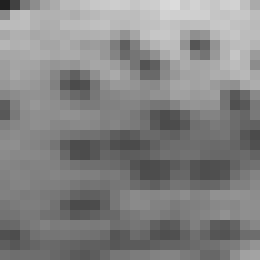
\includegraphics[width=1\textwidth]{compareImage/ORI_flowers_mag_G_2.png}
            \end{minipage}
        }
    \caption{ Comparisons between the FIRF methods and the proposed method. Ori is the original image. The proposed method recover more details, and its reconstructed image is much closer to the original image.}
    \label{fig:flower_gray}
\end{figure}
The SME method is sparse-coding based, and the FIRF method is interpolation based. The SME method must mix the outputs that are from many directional interpolators to generate the target output. The FIRF method consists of two phases. Each phase it must generate lots of SR decision trees. Furthermore, it has to fuse all the predicted values to generate the target value. Thus, both the SME method and FIRF method have a slower running speed in the reconstruction phase. The proposed method only constructs one SR decision tree, and it obtains the target value through one prediction. Thus, our method can achieve higher reconstruction accuracy with a faster running speed. The operation of fusion results in the smoothness in the reconstructed images of the SME method and FIRF method. There is no operation of fusion in our method. Thus, our reconstructed images are much clearer.

The LapSRN method’s network structure is too complicated. It trains a global non-linear mapping model, which describes the mapping relationship between the LR space and HR space. The deep complicated network makes a longer running time. The LapSRN method first extracts high-frequency information from the input LR image. Then, it upsamples the extracted high-frequency information, simultaneously the input LR image is upsampled. The sum of the two parts is the target output. The LapSRN methods upsamples the extracted high-frequency feature and the input LR image using a bilinear interpolation algorithm. The operation of interpolation makes the reconstructed images by the LapSRN method look much smoother. The proposed method doesn’t involve any operation of interpolation in both the training phase and the reconstruction phase. Thus, the proposed method can reconstruct clearer images.

\section{Conclusion}
ELM is fast learning algorithm for single-hidden-layer feedforward neural network. We propose a ELM-based single-image SR method. The proposed method performs the Hadamard transform on LR image patches to extract their Hadamard patterns (image feature). Our method classifies the training data based on the extracted Hadamard patterns. When the classification is complete, we learn a non-linear mapping model using ELM for each class. All the mapping models form a piecewise non-linear SR system. While classifying training data, an SR decision tree is constructed. Each leaf node corresponds to a mapping model. Experimental results show that the proposed method can achieve comparable reconstruction accuracy with a faster running speed.



%------------------------------------Conclusion-------------------------------

\section{Acknowledgments}

This work was partly supported by the National Science Foundation of China Grant 61300135, Pearl River Technology Nova Project Grant 201710010020, the Fundamental Research Funds for the Central Universities Grant x2rjD2153900, Hong Kong Scholars Program Grant XJ2014058, and the Open Project Program of the State Key Lab of CAD$\&$CG Grant A1619.

The authors would like to thank the editors and anonymous reviewers for their comments and suggestions.


\section*{References}

%\bibliographystyle{elsarticle-num-names}
\bibliography{mybibfile}
%% Harvard
\bibliographystyle{model2-names.bst}%\biboptions{authoryear}

\end{document} 